\subsection{Adjusted Mutual Information evolution over number points per dataset}
	
	These datasets have been created with 9 zernike modes.
	
	\subsubsection{AMI evolution for 500 points datasets}
		\begin{figure*}[ht!]
			\centering
			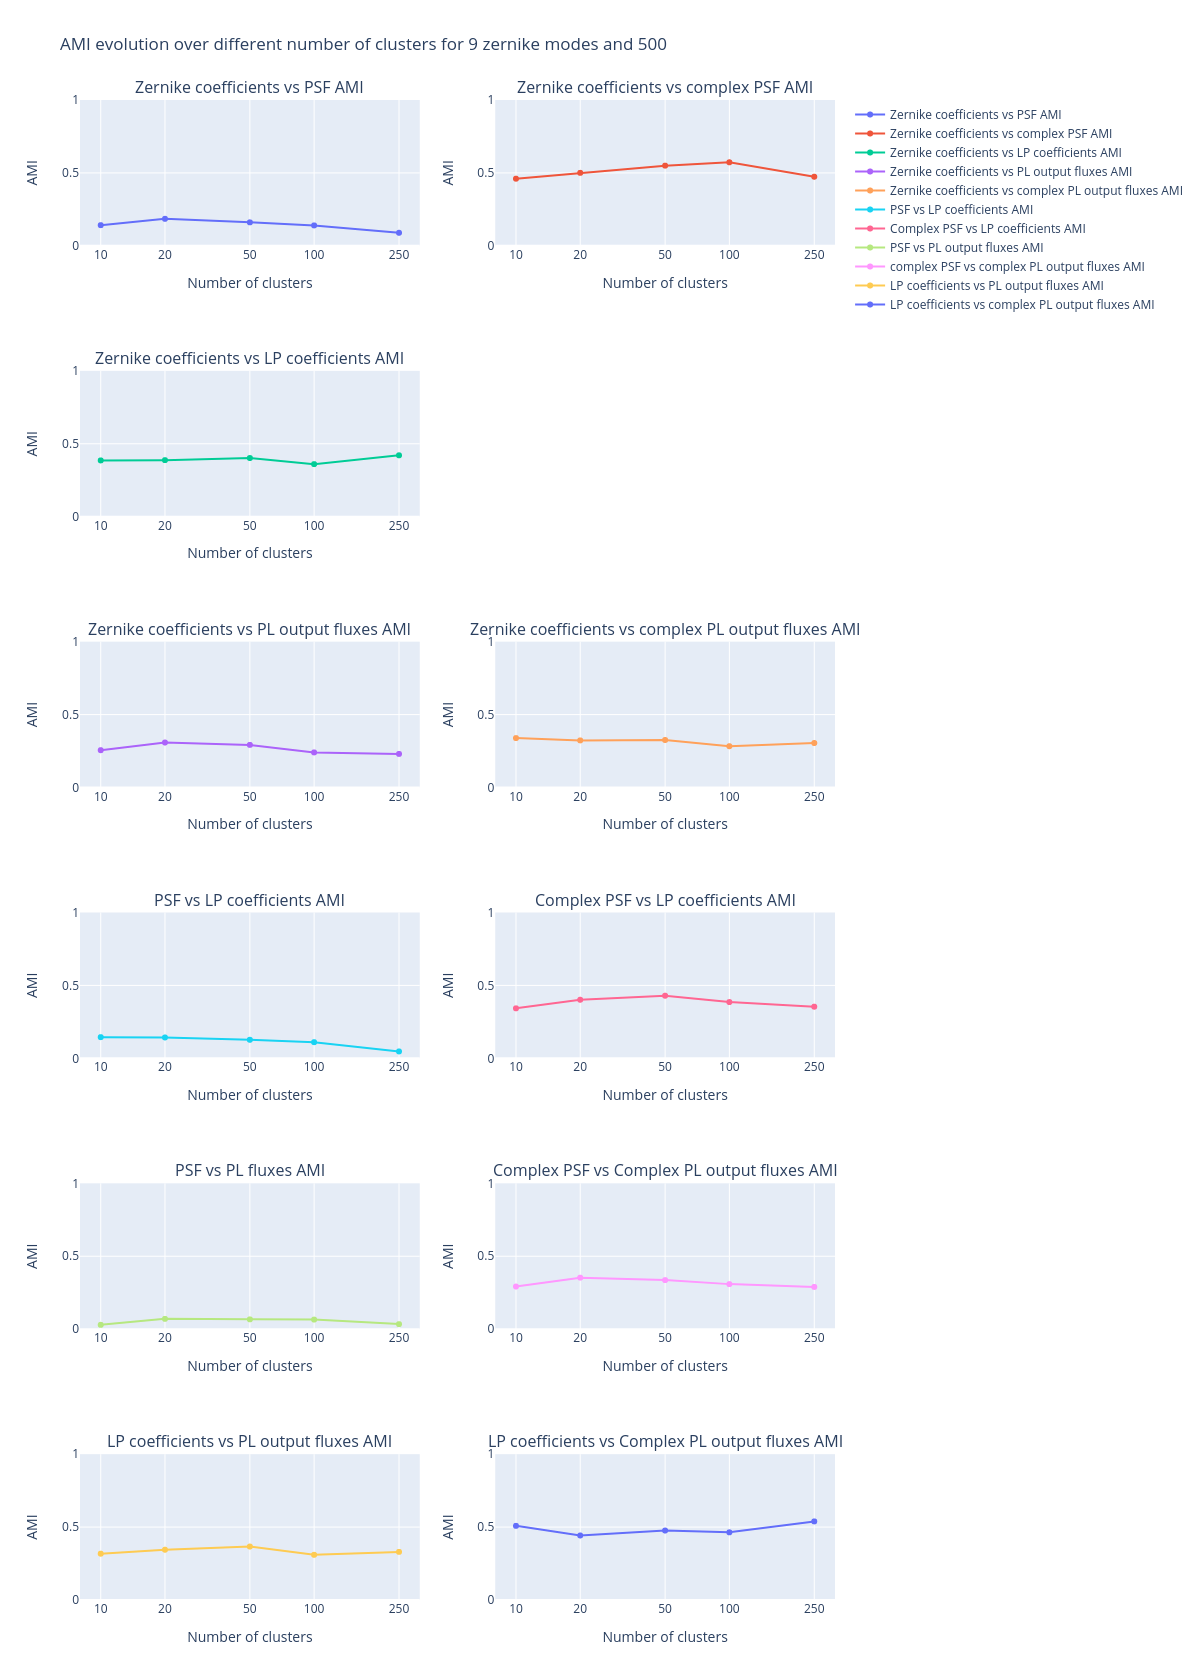
\includegraphics[width=0.7\textwidth]{ld-amievolutionover500.png}
		\end{figure*}
		\FloatBarrier
		
	\subsubsection{AMI evolution for 1000 points datasets}
		\begin{figure*}[ht!]
			\centering
			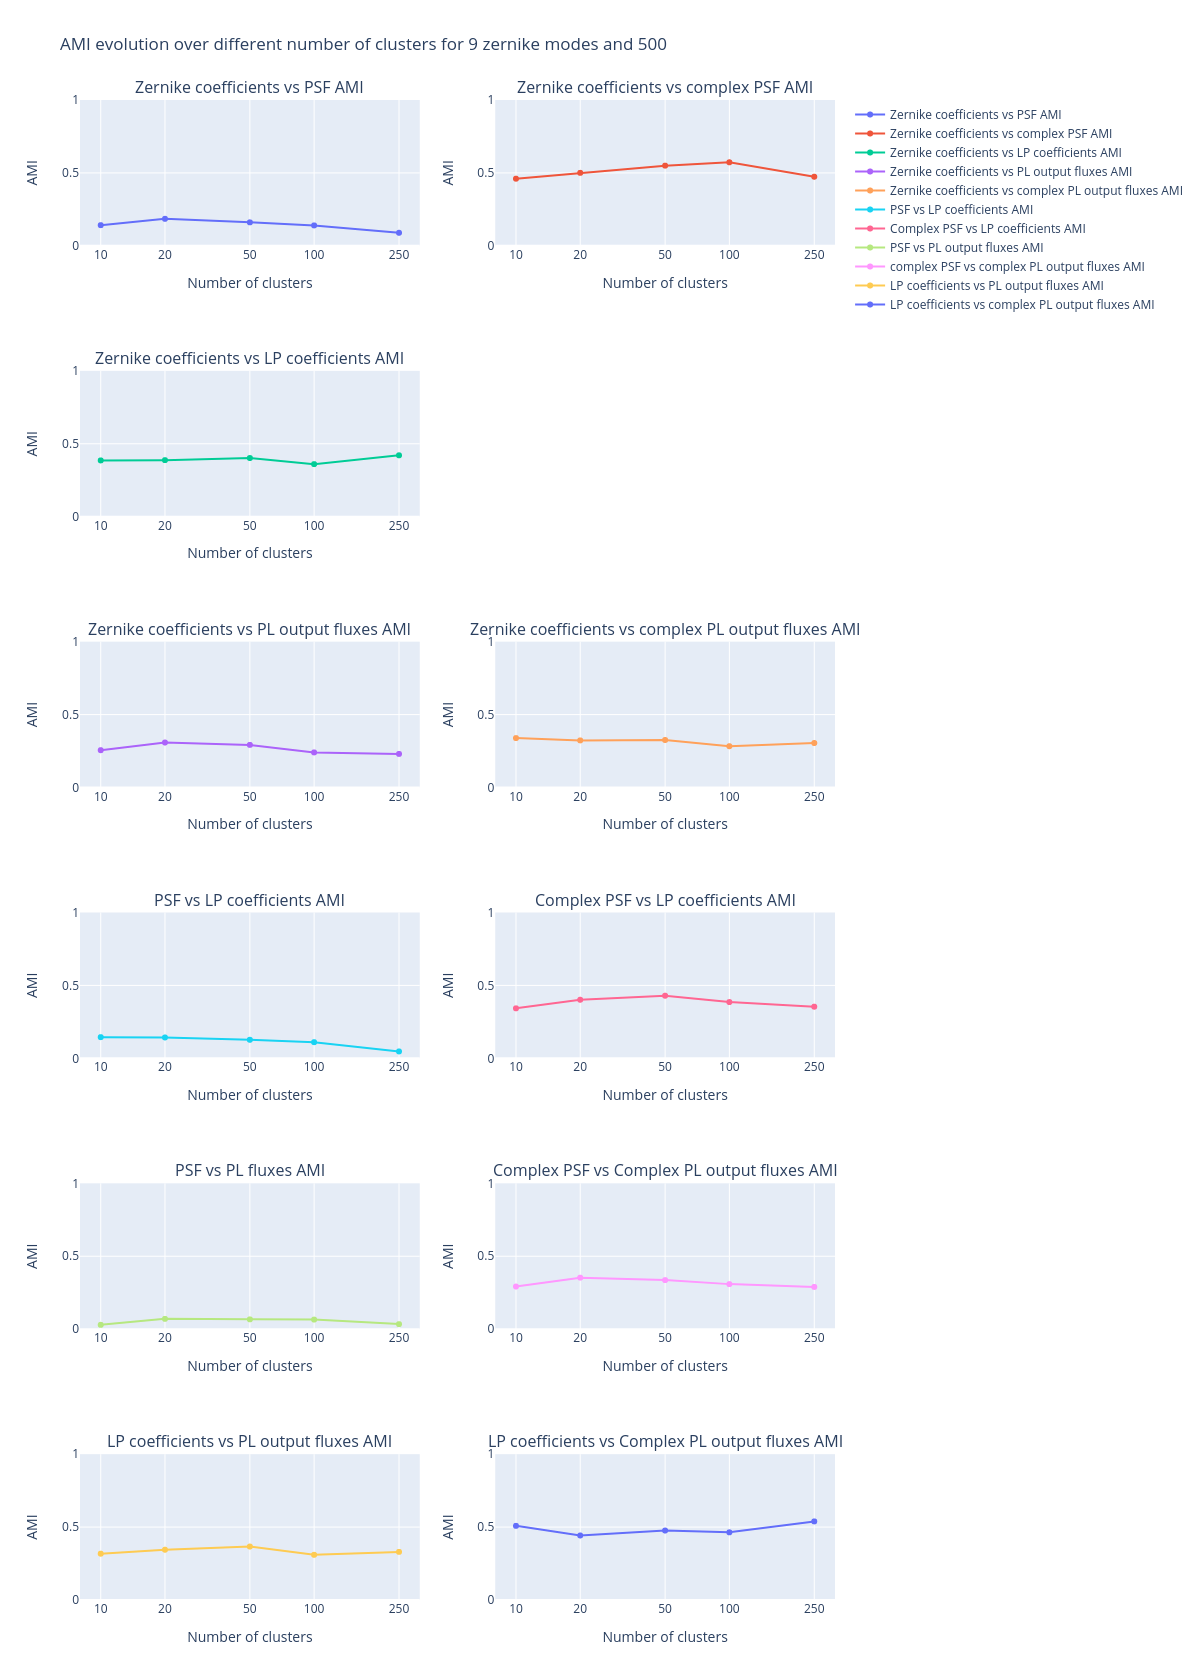
\includegraphics[width=0.8\textwidth]{ld-amievolutionover500.png}
		\end{figure*}
		\FloatBarrier
		
	\subsubsection{AMI evolution for 2000 points datasets}
		\begin{figure*}[ht!]
			\centering
			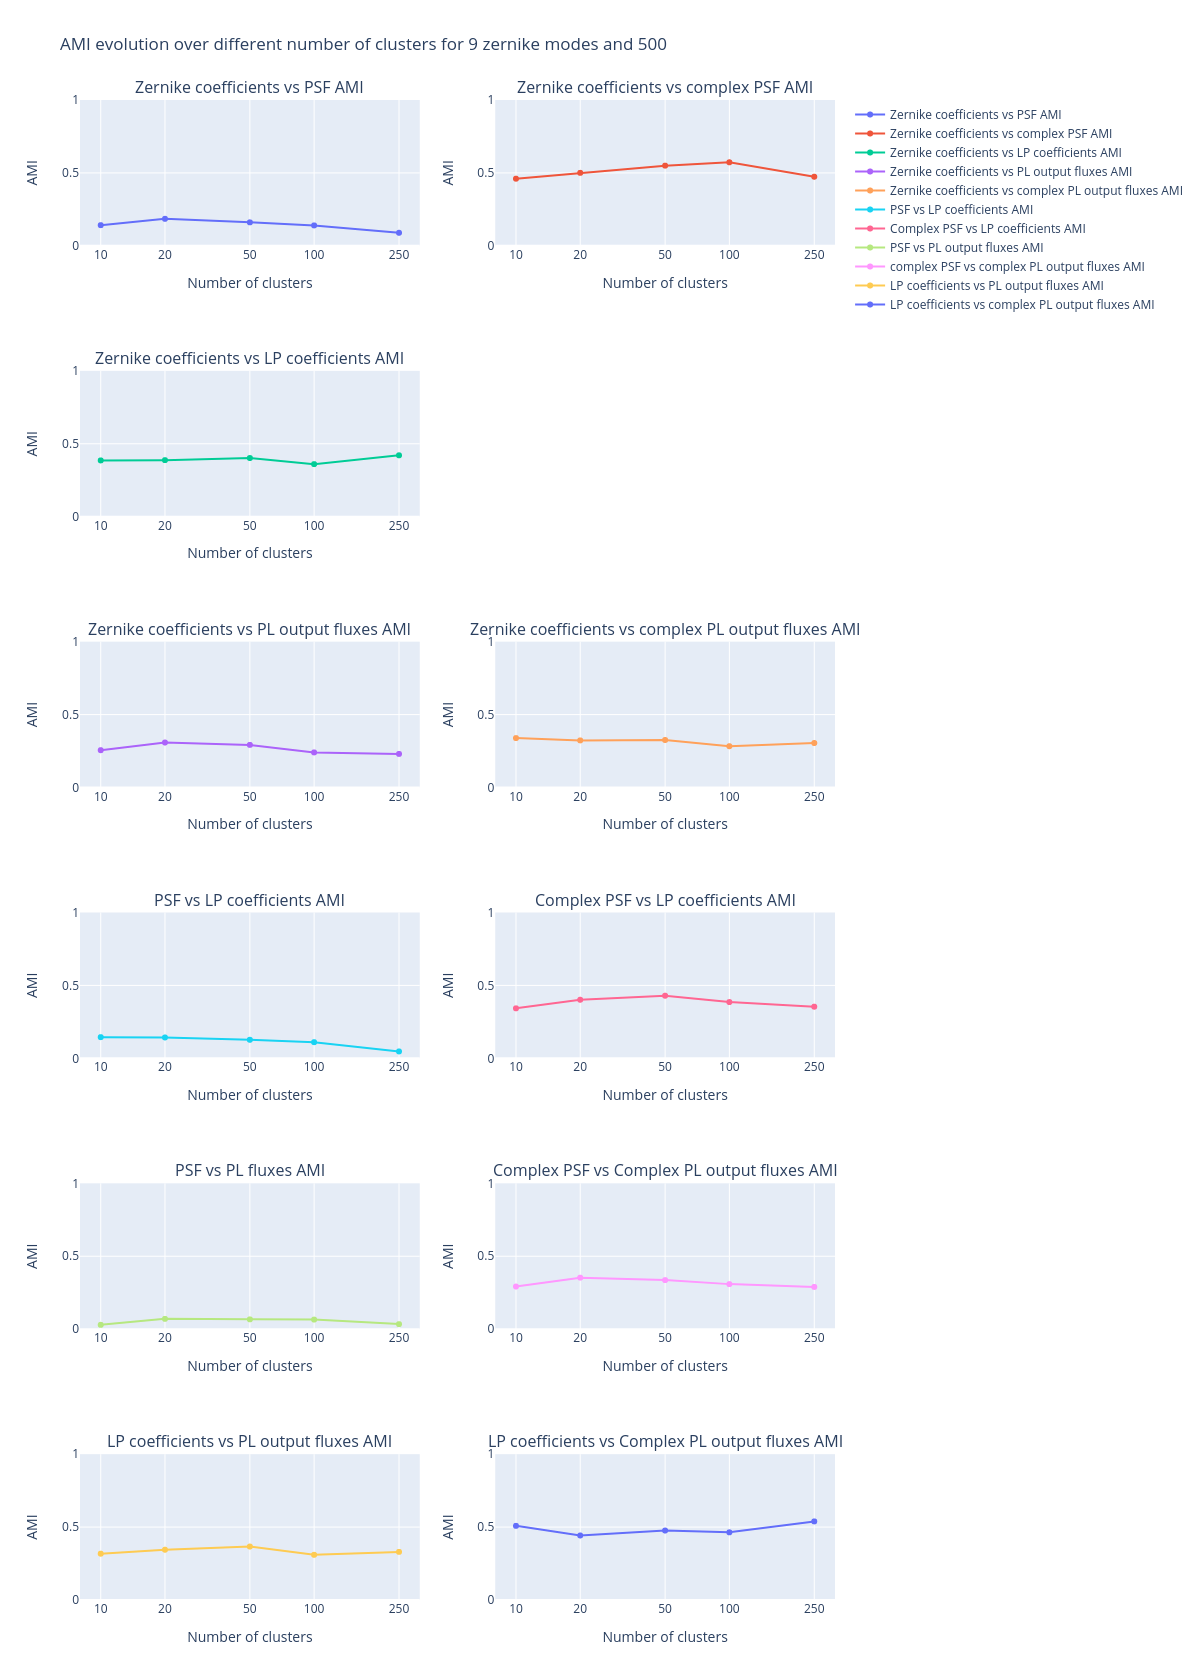
\includegraphics[width=0.8\textwidth]{ld-amievolutionover500.png}
		\end{figure*}
		\FloatBarrier
		
	\subsubsection{AMI evolution for 5000 points datasets}
		\begin{figure*}[ht!]
			\centering
			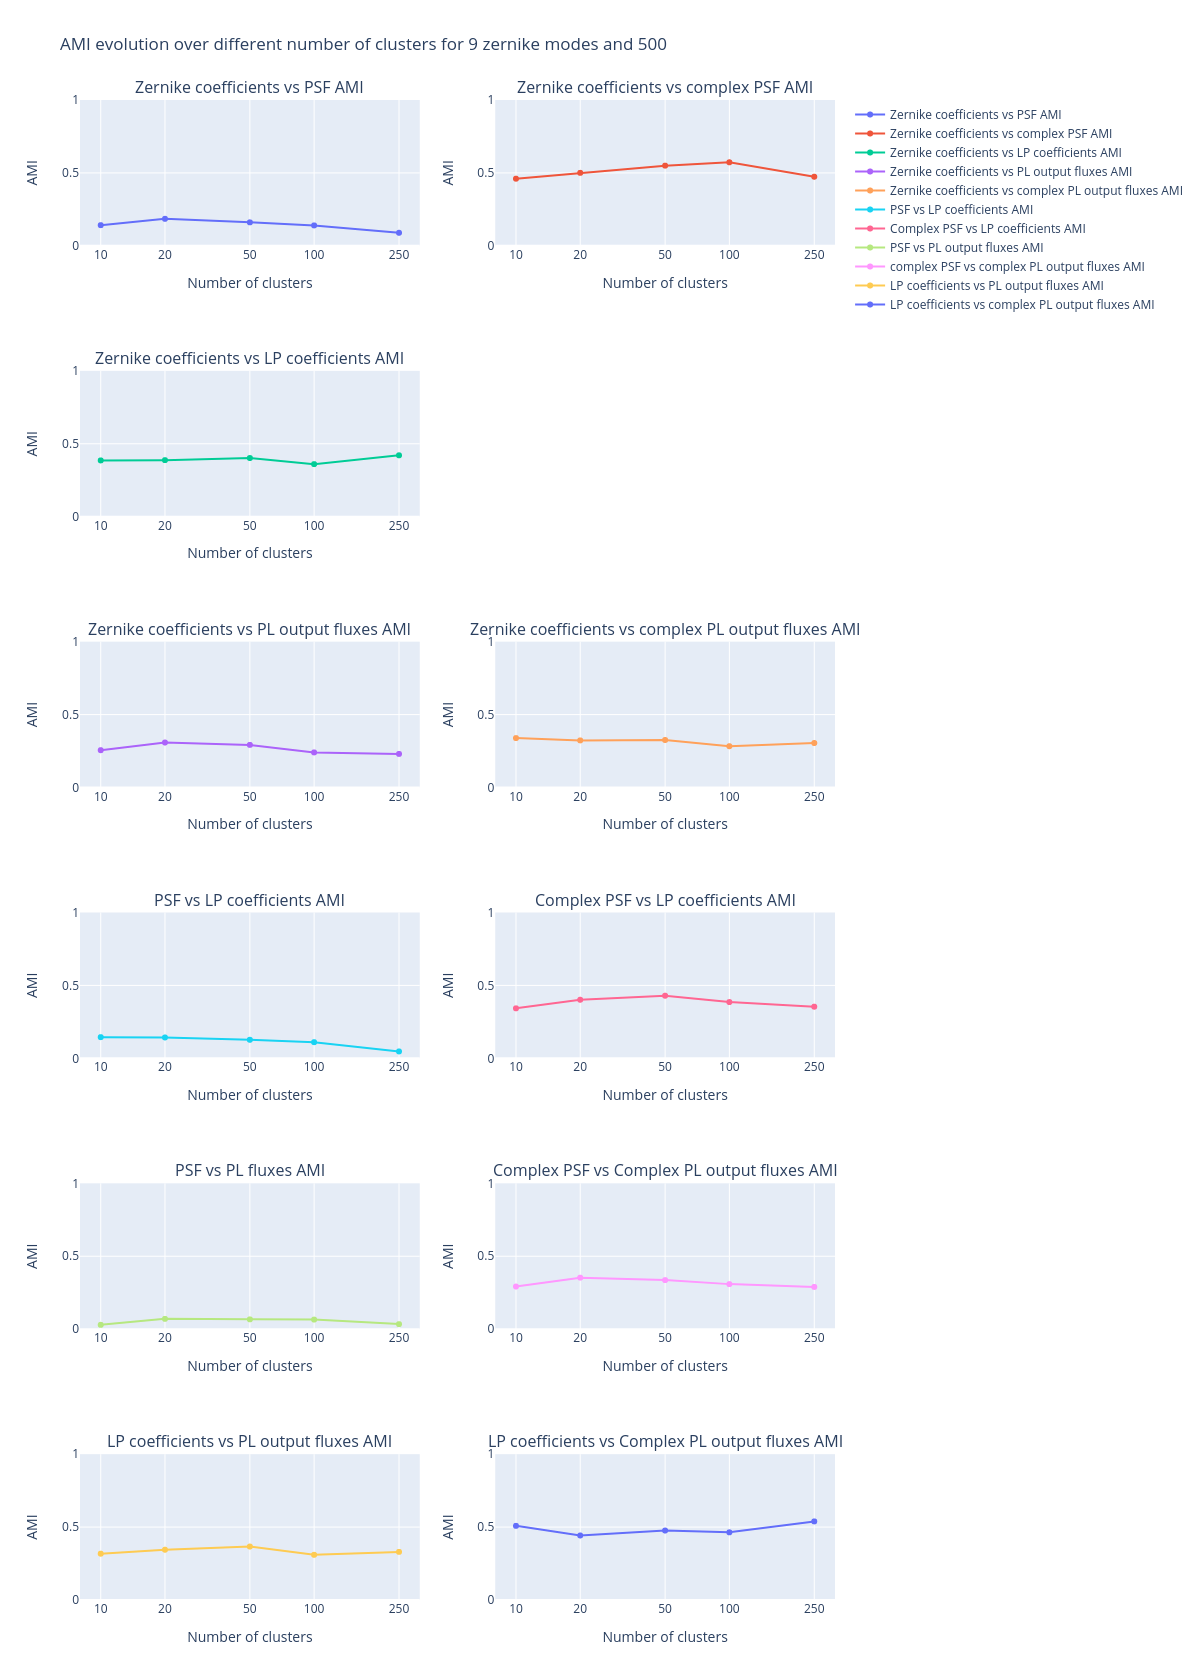
\includegraphics[width=0.8\textwidth]{ld-amievolutionover500.png}
		\end{figure*}
		\FloatBarrier
		
	\subsubsection{AMI evolution for 10000 points datasets}
		\begin{figure*}[ht!]
			\centering
			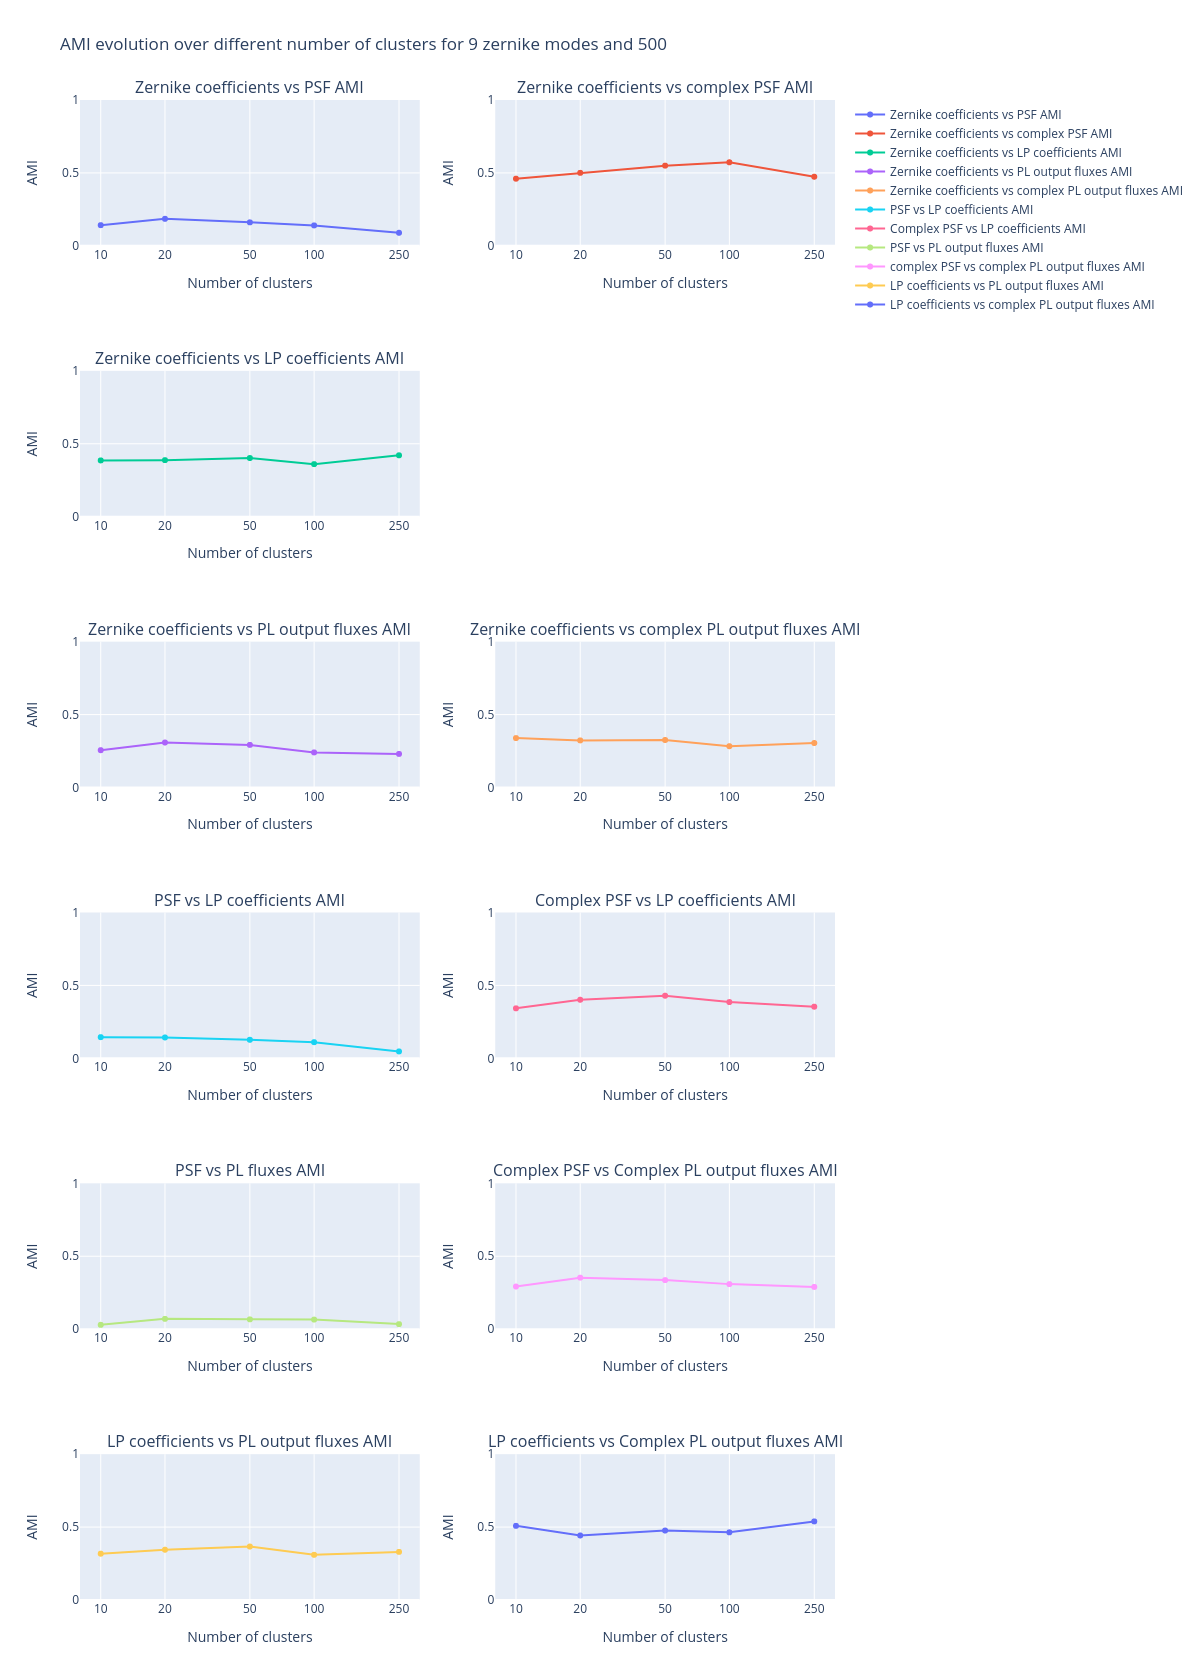
\includegraphics[width=0.8\textwidth]{ld-amievolutionover500.png}
		\end{figure*}
		\FloatBarrier
		
	\subsubsection{AMI evolution for 20000 points datasets}
		\begin{figure*}[ht!]
			\centering
			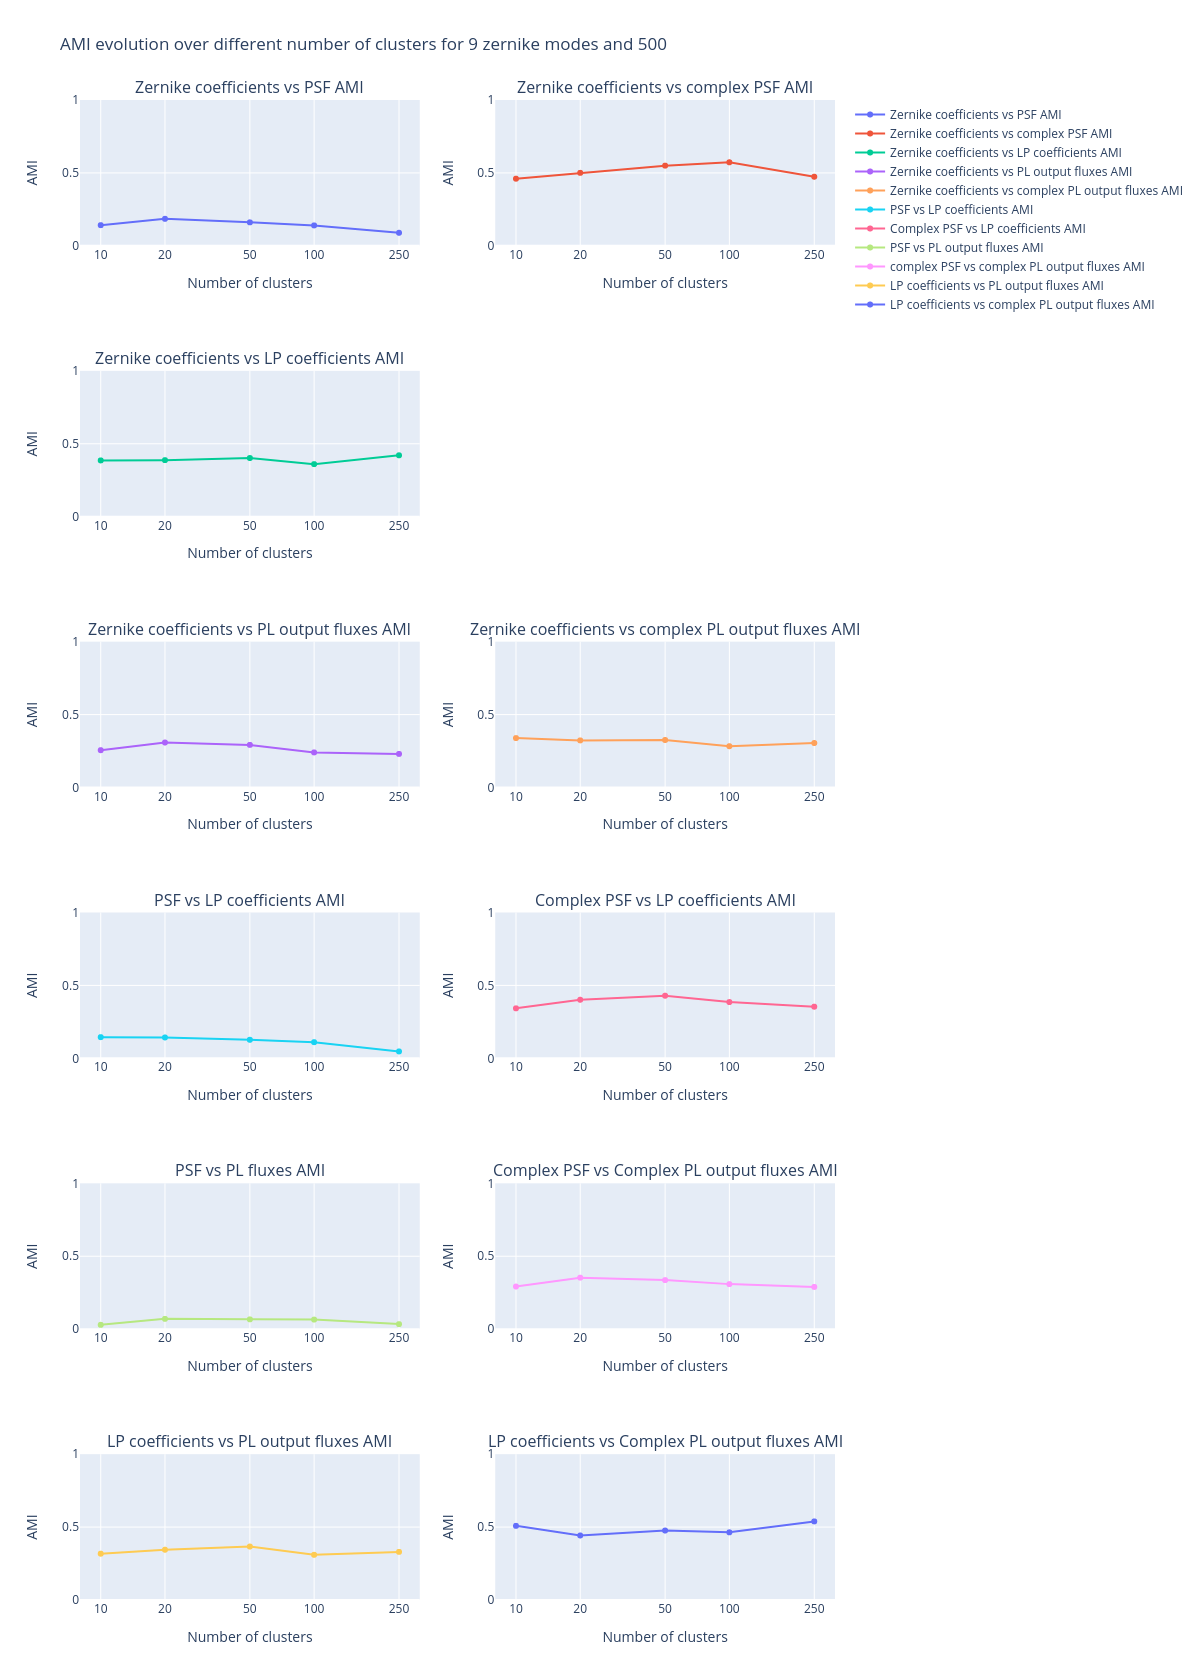
\includegraphics[width=0.8\textwidth]{ld-amievolutionover500.png}
		\end{figure*}
		\FloatBarrier
		
	\subsubsection{Maximum AMI for the datasets}
		\begin{figure*}[ht!]
			\centering
			\subfloat[AMI evolution over number of clusters for Zernike coefficients vs PSF]{%
				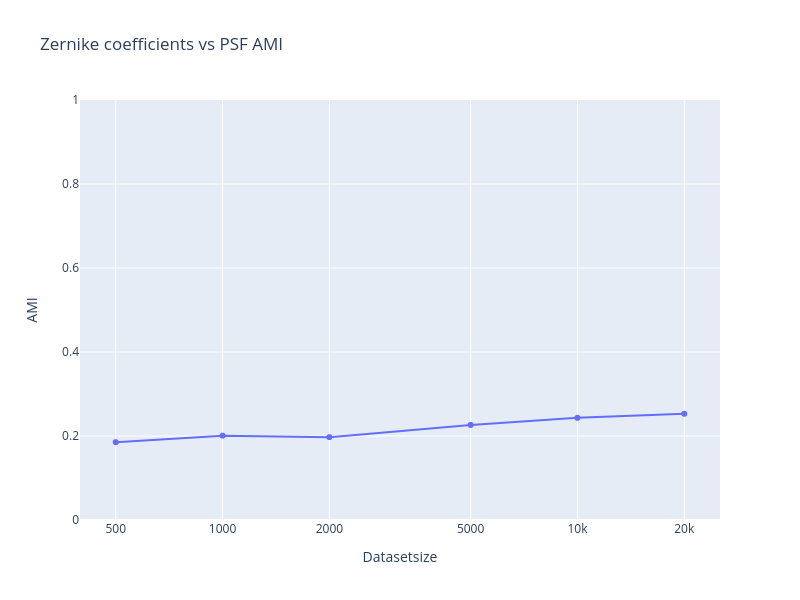
\includegraphics[width=0.45\textwidth]{ld-zernikecoefficientsvspsfami.png}}
			\hspace{\fill}
			\subfloat[AMI evolution over number of clusters for Zernike coefficients vs LP coefficients]{%
				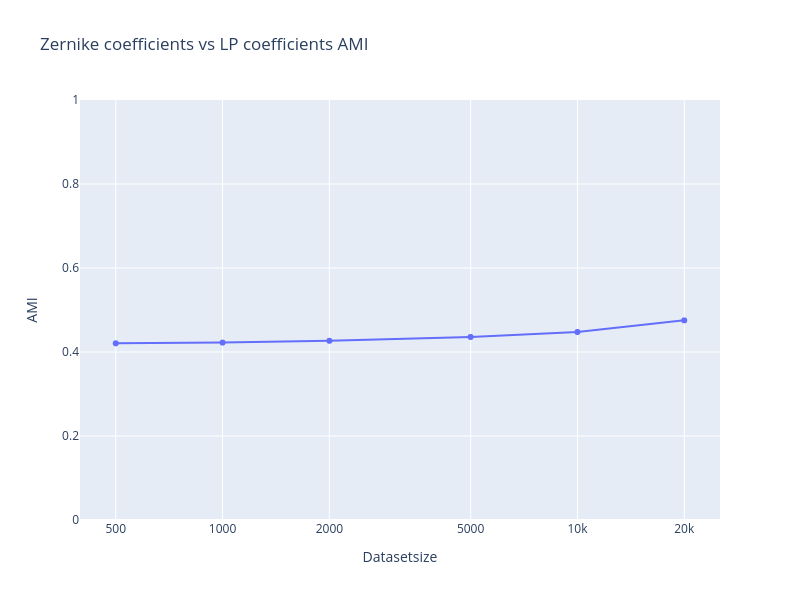
\includegraphics[width=0.45\textwidth]{ld-zernikecoefficientsvslpcoefficientsami.png}}
			\\
			\subfloat[AMI evolution over number of clusters for Zernike coefficients vs PL output fluxes]{%
				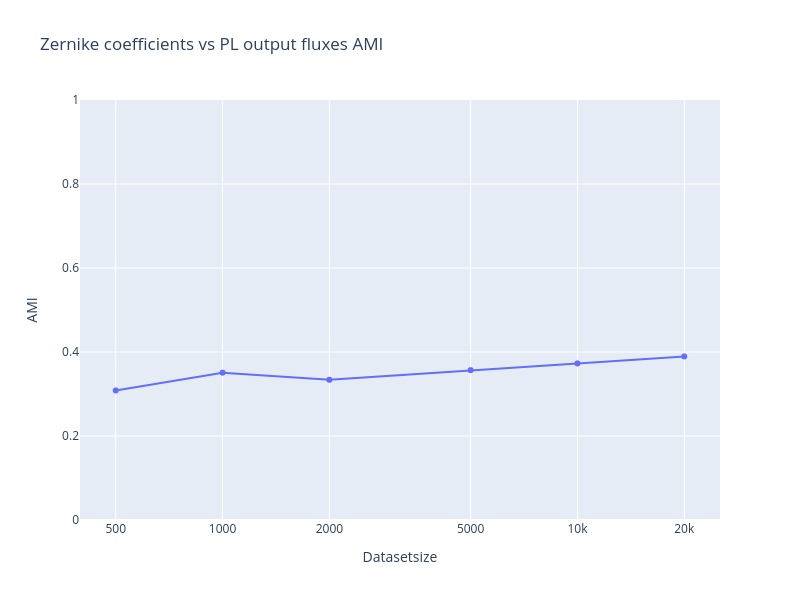
\includegraphics[width=0.45\textwidth]{ld-zernikecoefficientsvsploutputfluxesami.png}}
			\hspace{\fill}
			\subfloat[AMI evolution over number of clusters for PSF vs LP coefficients]{%
				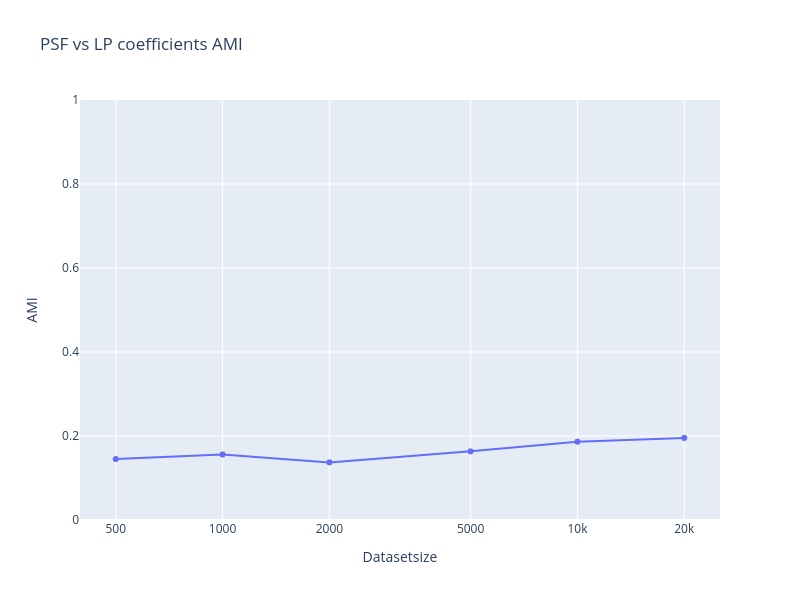
\includegraphics[width=0.45\textwidth]{ld-psfvslpcoefficientsami.png}}
			\\
			\subfloat[AMI evolution over number of clusters for PSF vs PL output fluxes]{%
				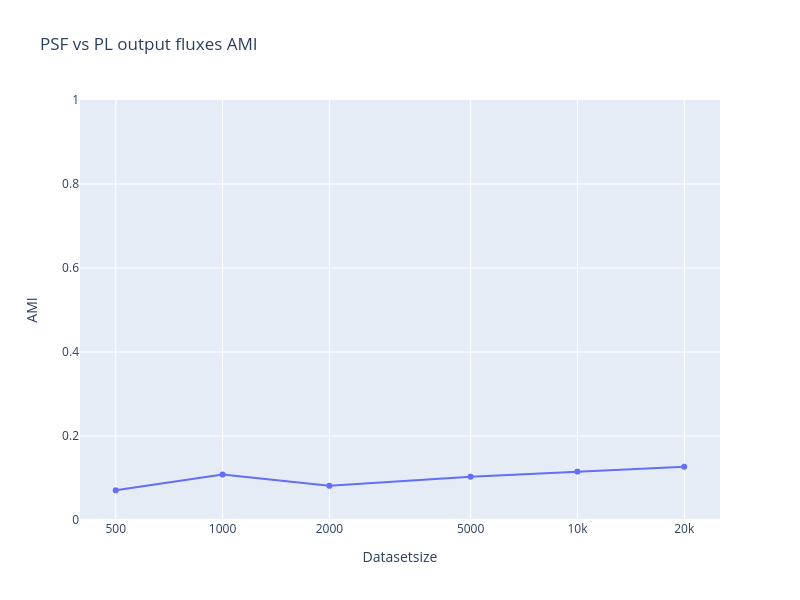
\includegraphics[width=0.45\textwidth]{ld-psfvsploutputfluxesami.png}}
			\hspace{\fill}
			\subfloat[AMI evolution over number of clusters for LP coefficients vs PL output fluxes]{%
				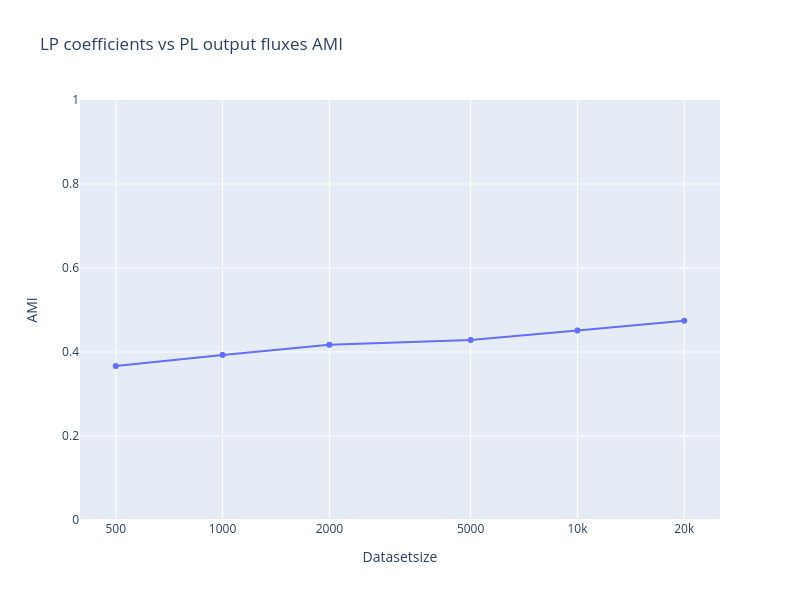
\includegraphics[width=0.45\textwidth]{ld-lpcoefficientsvsploutputfluxesami.png}}
		\end{figure*}
		
		\begin{figure*}[ht!]
			\centering
			\subfloat[AMI evolution over number of clusters for Zernike coefficients vs complex PSF]{%
				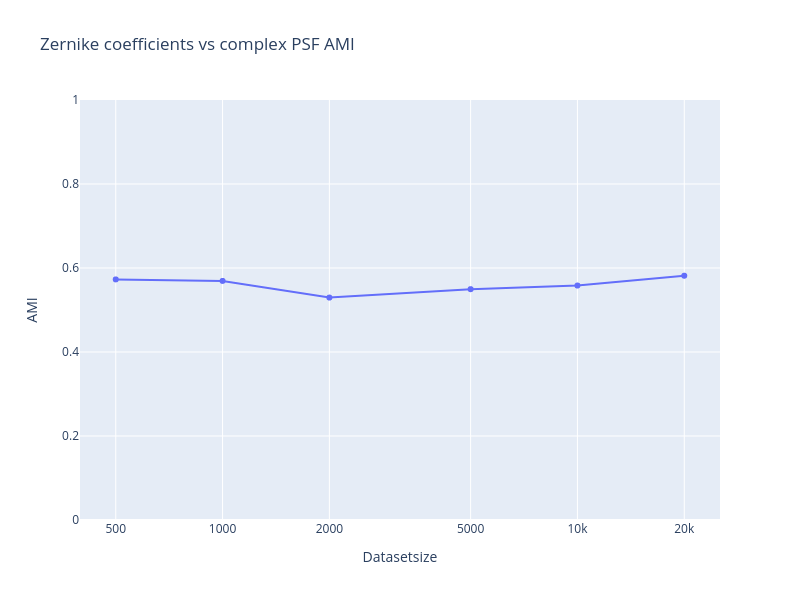
\includegraphics[width=0.45\textwidth]{ld-zernikecoefficientsvscomplexpsfami.png}}
			\hspace{\fill}
			\subfloat[AMI evolution over number of clusters for Zernike coefficients vs complex PL output fluxes]{%
				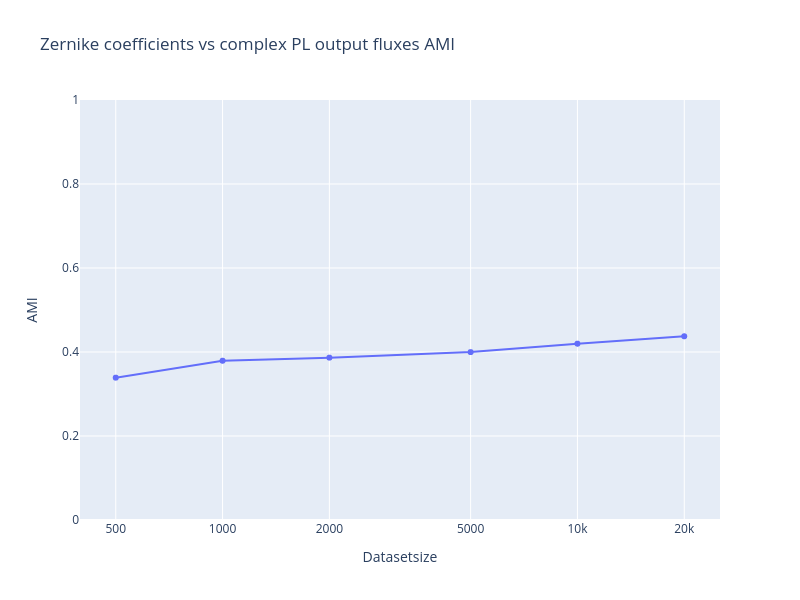
\includegraphics[width=0.45\textwidth]{ld-zernikecoefficientsvscomplexploutputfluxesami.png}}
			\\
			\subfloat[AMI evolution over number of clusters for complex PSF vs LP coefficients]{%
				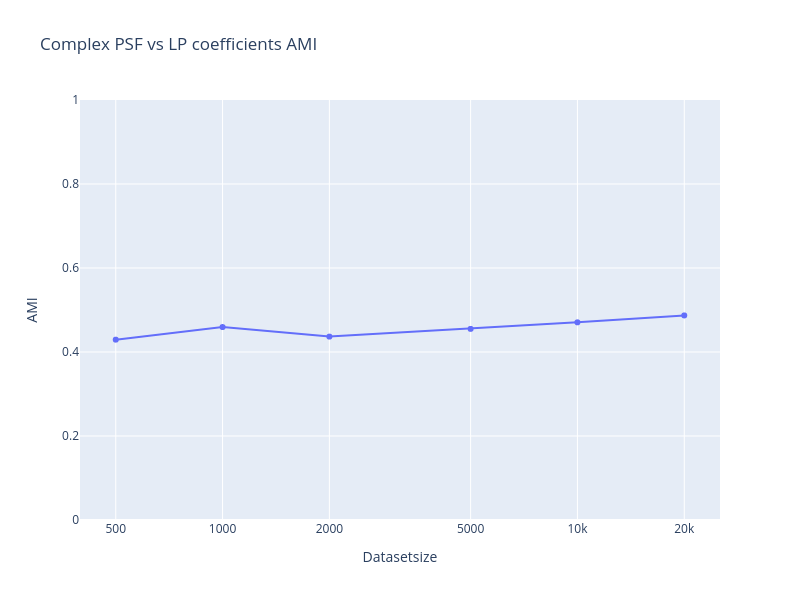
\includegraphics[width=0.45\textwidth]{ld-complexpsfvslpcoefficientsami.png}}
			\hspace{\fill}
			\subfloat[AMI evolution over number of clusters for commplex PSF vs complex PL output fluxes]{%
				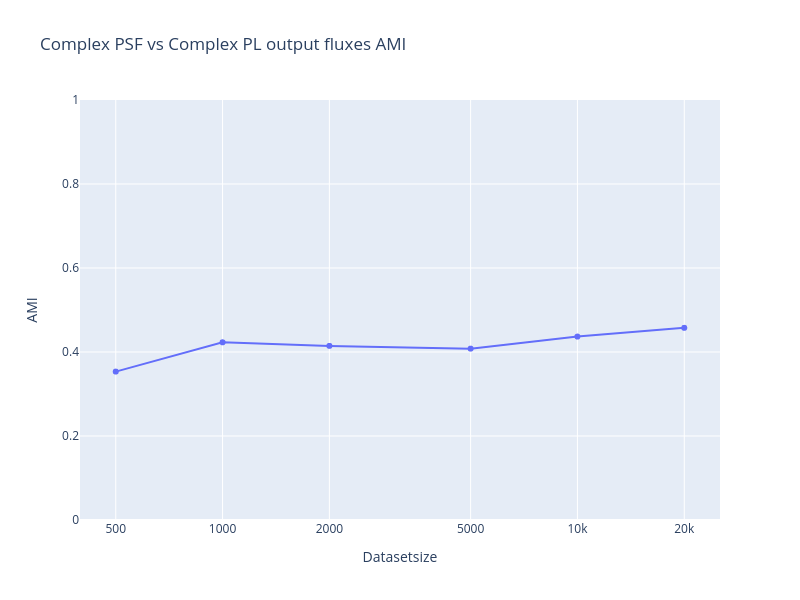
\includegraphics[width=0.45\textwidth]{ld-complexpsfvscomplexploutputfluxesami.png}}
			\\
			\subfloat[AMI evolution over number of clusters for LP coefficients vs complex PL output fluxes]{%
				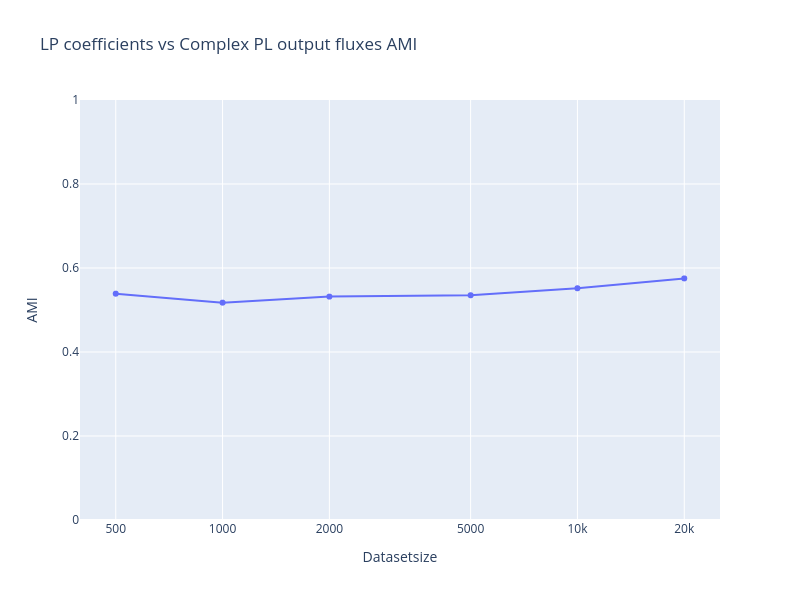
\includegraphics[width=0.45\textwidth]{ld-lpcoefficientsvscomplexploutputfluxesami.png}}
		\end{figure*}

		\FloatBarrier